\documentclass[parskip,
  oneside,
  % longdoc,
  11pt,
  noheadingspace,
  accentcolor=tud1d,
  bigchapter,
  % draft,
  colorback]{tudreport}

\usepackage[utf8]{inputenc}
\usepackage[english]{babel}
\usepackage{acronym}
\usepackage{tabularx}
\usepackage{url}
\usepackage{hyperref}
\usepackage{siunitx}
\usepackage{xcolor}
\usepackage{listings}
\usepackage{rotating}

\usepackage[%
  backend=bibtex      % biber or bibtex
 ,style=alphabetic    % Alphabeticalsch
 %,style=numeric-comp  % numerical-compressed
 ,sorting=none        % no sorting
 ,sortcites=true      % some other example options ...
 ,block=none
 ,indexing=false
 ,citereset=none
 ,isbn=false
 ,url=true
 ,doi=true            % prints doi
 ,natbib=true         % if you need natbib functions
]{biblatex}

\addbibresource{bib.bib}  % better than \bibliography

\makeatother

\title{\textbf{Rechnersysteme II Erste Übung}}
\subtitle{Ausarbeitung vorgelegt von Ela, Marcel}
\subsubtitle{Betreuer: Dipl.-Ing. (Name des Betreuers)\\
       Beginn: (Beginndatum) \textbar\ Abgabe: (Abgabedatum)\\
       Institut f\"ur Datentechnik\hfill\textbar\hfill Fachgebiet Rechnersysteme\hfill\textbar\hfill Prof.\,Dr.-Ing.\, Christian Hochberger}
\setinstitutionlogo{images/logo.pdf}

\begin{document}

%% Titel %%%%%%%%%%%%%%%%%%%%%%%%%%%%%%%%%%%%%%%%%%%%%%%%%%%%%%%%%%%%%%
\maketitle
\cleardoublepage

%% Vorgeplenkel %%%%%%%%%%%%%%%%%%%%%%%%%%%%%%%%%%%%%%%%%%%%%%%%%%%%%%%%
\pagestyle{empty}

%% Main %%%%%%%%%%%%%%%%%%%%%%%%%%%%%%%%%%%%%%%%%%%%%%%%%%%%%%%%%%%%%%%
\pagestyle{headings}
\pagenumbering{arabic}
  \chapter{Introduction}
\label{cha:intro}
	During the lecture "Rechnersysteme II" students are able to take part in an exercise about System on Chip (SoC) Kits. These kits provide the user with a tool chain to seamlessly integrate software and hardware components in a single system on a single chip. The SoC Kit in use is based on the SpartanMC processor, which was developed to be implemented in the context of FPGAs making optimal use of their resources.

	The main assignment of the exercise is to implement a distance meter using an ultrasonic sensor and an OLED display to visualise the measured data. Multiple tasks are provided to get to know and integrate the required peripherals step by step. Software has to be written for communicating with the ultrasonic sensor (SRF02) and the OLED display, which are integrated into the overall system by using jConfig. Each peripheral uses its own serial bus interface (I2C and SPI).

	Bonus tasks revolve around implementing an interrupt based solution for the bus interface drivers of the ultrasonic sensor and the OLED display. Further more, code profiling of two procedures and verification of their runtime behaviour is part of the set of additional tasks.

	All tasks, including the bonus tasks, of the exercise were handled during the curse of solving it.
  \chapter{Task Description}
\label{cha:task}

bla
  \chapter{Implementation} % (fold)
\label{cha:impl}
	Just like in the previous chapter [\ref{cha:task}], every task will have its implementation process described in its own section.

	\section{Task I} % (fold)
	\label{sec:impl_task_1}
		The implemented system consists of an UART Light peripheral as well as an I2C Master. More details concerning these two will be given in the following sub sections. A third sub section describes the implementation of a filter which shall detect erroneous data.
	
		\subsection{UART Light} % (fold)
		\label{sub:uart_light}
			In JConfig, we selected the UART Light Bus from the peripheral modules, setting a baudrate of 115200 and the same clock as the Spartan MC core. After mapping the stdout FILE to the UART Light peripheral, it is now possible to use the standard libraries IO procedures which are implemented for SpartanMC to send any textual information back to the development computer.
			Using printf(), we send the data measured by the sensor to the computer, where we read it from /dev/ttyUSB0.
		% subsection uart_light (end)

		\subsection{I2C Master} % (fold)
		\label{i2c_master}
			In this task, a basic implementation of I2C was designed, without making use of interrupts. First, I2C was added in JConfig and the SDA and SCL signals were connected to the pins of the FPGA according to the FPGA pin sheet.
			In order to fulfil the task, the following procedures were implemented, besides the main procedure:
			
			\begin{itemize}
				\item sensor\_enable(i2c\_master\_regs\_t* i2c, int prescaler)
				\item sensor\_send(i2c\_master\_regs\_t* i2c, const unsigned char ch, const int slv\_addr, const int reg)
				\item sensor\_read(i2c\_master\_regs\_t* i2c, const int slv\_addr, const int reg)
		   	\end{itemize}
			
			\paragraph{Enable and Configuration} % (fold)
	   		\label{par:enable_task1}
   				The "sensor\_enable" procedure sets the bits of the control register, in order to establish a correct I2C connection. The I2C core is enabled by setting the CORE\_EN bit. Additionally, the right frequency of the SCL line is chosen by assigning the prescaler with the correct value. In the main procedure, this corresponds to a frequency of \SI{40}{\kilo\hertz}, which was computed using the formula:  prescaler = (peripheral\_clock /(5 * desired\_SCL)) -1
			% paragraph enable_task1 (end)
				
			\paragraph{Data Write} % (fold)
	   		\label{par:data_write_task1}
	   			A write access, which occurs when calling the "sensor\_send" procedure, must contain the ID of the slave, the register number where the data will be written and the information to be sent. The transfer is initiated by setting the STA bit and the number of transferred bytes. When computing this value, counting the bytes sent as useful data is not enough. The COUNT value takes into consideration also the bytes containing the slave address and the register number.
				We use this procedure to tell the sensor to start ranging in centimetres. This means that we write the value \num{81} to register zero.
			% paragraph data_write_task1 (end)
			
			\paragraph{Data Read} % (fold)
	   		\label{par:data_read_task1}
	   			The read access starts with a write of two bytes, telling the sensor the register number from which we want to receive data. Afterwards, a read request is initiated, by setting the last bit of the slave ID. Additionally, the RD bit of the Command register is one. The COUNT value is now three, which means that one byte will be written (the slave ID) and two bytes are requested. The number of demanded bytes comes from the fact that the result is split in the registers two and three of the sensor and has \num{16} bits. The result is than read from the I2C data register and the STO bit of the command register is set.
			% paragraph data_read_task1 (end)
			
			\paragraph{Main procedure} % (fold)
	   		\label{par:data_read_task1}
	   			As stated above, the main procedure sets a frequency of \SI{40}{\kilo\hertz} for the SCL line, by calling the sensor\_enable function. Subsequently, it tells the sensor to start measuring in centimetres. A delay (greater \SI{65}{\milli\second}, as per the sensors manual) was implemented to wait for the SRF02 to finish ranging. Afterwards, the result is read through the I2C and sent to the computer via the UART Light. This is done in an endless loop.
			% paragraph data_read_task1 (end)
		% subsection i2c_master (end)

		\subsection{Filtering of acquired data} % (fold)
		\label{sub:filter}
			In order to filter the information obtained from the distance measuring sensor, a comparison to the previously received data must be conducted. Thus, storing part of the measured data is necessary.
			This project proposes a simple implementation of such a filter by storing ten measured values and comparing their mean to the new data. If the latest measurement is greater or smaller than the mean by 50 units, than the value is not printed. However, it is stored. When the program starts, no value is already available, thus the first one is printed without any filtering. In case the first value was incorrect, the filter will converge to a good result after some measurements.
			This approach was easy and fast to implement and returns good results for this type of application. If a high reliable result was required, then the Kalman filter could have been a good replacement. When using such an approach, the behaviour of the sensor must be described.
		% section filter (end)
	% section task_1 (end)

	\section{Task II} % (fold)
	\label{sec:impl_task_2}
		Communication with the OLED display is to be facilitated by using an SPI master, which has to be added to the jConfig project. Connecting the SPI master instance to the required FPGA pins is straight forward as the required connections (CS, SCLK, SDIN, RES) are denoted by the the provided FPGA pin sheet. However, the displays' reset pin requires a separate output port instance to be generated by jConfig and can not be connected directly to the SPI master peripheral. 

		\subsection{SPI Implementation} % (fold)
		\label{sub:impl_spi_implementation}
			Implementing the SPI driver is split into three parts:

			\begin{itemize}
				\item SPI enable and initial configuration
				\item SPI slave de-/select
				\item SPI data write
	   		\end{itemize}

	   		Each listed item will be described in one of the following paragraphs and relates to similarly name procedures in the main source file.

	   		\paragraph{Enable and Configuration} % (fold)
	   		\label{par:enable}
	   			Enabling and configuring the SPI master is implemented by writing to its control register. The task description states that the serial clock of the SPI connection has to be set to under \SI{10}{\mega\hertz}. This is achieved by setting the clock divider to two, resulting in a frequency of \SI{7.5}{\mega\hertz}, following the equation given in the SpartanMC manual. The bit width for each transfer is retrievable from the displays SPI manual and the fact that we will be using the described three wire interface, relying only on the serial data pin to send commands and data to the display. Reading further in the manual shows that eight bits plus one mode selection (command/data) bit are part of each transfer, making this nine bit in total. As a result of these observations, the value nine is written to the BITCNT property of the control register. Lastly, the enable bit is set, completing the initial configuration procedure.
	   		% paragraph enable (end)

	   		\paragraph{Slave De-/select} % (fold)
	   		\label{par:slave_de_select}
	   			Selecting the SPI slave targeted by the master requires a read to its control register. As the only available slave is attached to the first slave select signal, this value will be set one time before using the SPI interface and remains the same for the duration of the whole program.
	   		% paragraph slave_de_select (end)

	   		\paragraph{Data Write} % (fold)
	   		\label{par:data_write}
	   			As there is no need to retrieve data from to display, the write implementation will suffice to be able to use it. Writing to the masters data output register and waiting for all bits to be sent is the only thing to do. This first (but also the final I2C interrupt driven) implementation is polling the fill bits of the status register until the retrieved value is zero, denoting an empty output register and the ability to send more data.
	   			It is notable that the nine bits (one selecting command/data mode and eight with actual payload) to send are composed in such a way that the mode selection bit is the highest one.
	   		% paragraph data_write (end)
		% subsection impl_spi_implementation (end)

		\subsection{Display Driver Cleanup} % (fold)
		\label{sub:impl_display_driver_cleanup}
			As source code for the display driver is already provided, it remains to adjust it to our system. This includes the replacement of the data and command transaction routine implementations with own code calling the SPI procedures, but extends to the not compiling driver code. The latter is caused by multiple missing type declarations of local variables but also by the not defined global variable "Shift". Further errors are generated by the missing inclusion of the font header and by undefined GPIO related macros. As all GPIO accesses can be replaced by SPI or the newly introduced reset output port, no undefined variables and macros remain.

			\paragraph{ASCII Table} % (fold)
			\label{par:ascii_table}
				The recently mentioned font header provides data for printing ASCII characters to the display. However, when trying to write string literals to the display it can be observed that the provided table is shifted by an offset of minus \num{32}. Simply adding this value to each index used in the Show\_Font57\_25664 procedure resolves this issue.
			% paragraph ascii_table (end)

			\paragraph{Global Shift} % (fold)
			\label{par:global_shift}
				A global variable called "Shift" is used to place correctly the text on the horizontal axis of the display. Experimentally, we set this variable to the value \num{28}. 
			% paragraph global_shift (end)
		% subsection display_driver_cleanup (end)

		\subsection{Display Usage} % (fold)
		\label{sub:display_usage}
			Before using the display it is required to configure the SPI master and initialise the display with the already available OLED\_Init\_25664 procedure. Afterwards, the displays' RAM is initialised to ensure a none noisy background.
			Printing strings to the display is achieved by a call to Show\_String\_25664. At this point it is possible to combine the sensor data retrieval with the display and solve the third task.
		% subsection display_usage (end)
	% section task_2 (end)

	\section{Task III} % (fold)
	\label{sec:impl_task_3}
		We are now able to print strings on the OLED display and to read data measured by the sensor. The updates required to combine these functionalities are presented in the following subsections.
		
		\subsection{Integer to String Conversion} % (fold)
		\label{sub:integer_to_string_conversion}
			The data read from the sensor is stored as an integer value. To print it on the OLED display, we implemented a procedure that converts an integer to a string: "int\_to\_str". Each cipher of the number is evaluated, and a string is constructed accordingly. The procedure can convert a number less than 1000. If the first cipher is a zero, it is replaced by a space character when building the string. Since the sensor can measure at least \SI{15}{\centi\meter}, there is no need to replace the zeroes on the second position.  
		% subsection integer_to_string_conversion (end)

		\subsection{Integration} % (fold)
		\label{sub:integration}
			The two functionalities are combined in a new main procedure. The SPI peripheral, namely the OLED display, is enabled and a delay is inserted to wait for this process to complete. Some data regarding the control and status registers is sent via UART for debug purposes. After the SPI slave is selected, the display and its RAM are initialized by calling the "OLED\_Init\_25664" and "Clear\_RAM" procedures. Using the procedure "Show\_String\_25664", the text "Der Abstand ist: " is printed and emphasized through dashed lines. 
			In an endless loop, the procedure "sensor\_read" is called. This starts a new measurement in centimetres, and after a delay of approximately 
			\begin{math} 
				1000 \times 6000 \times 3 
			\end{math} 
			clock cycles, which results in a delay of around \SI{300}{\milli\second}, the result is read from the sensor. This delay is sufficient for the sensor, which according to the data sheet is able to measure in \SI{65}{\milli\second}. To save some time, we can divide the value given to the sleep procedure by three, as this will still suffice. The value read from the sensor is converted to a string and is printed on the display. It appears after the text "Der Abstand ist: ", thus an adjustment of the horizontal offset was needed.
		% subsection integration (end)
	% section task_3 (end)

	\section{Bonus Task I} % (fold)
	\label{sec:impl_bonus_task_1}
		Starting with initial thoughts on possible gains and costs for choosing SPI or I2C as the optimisation target, this section describes how the first bonus task was solved and which problems were encountered.

		\subsection{Initial Considerations} % (fold)
		\label{sub:initial_considerations}
			The first important question for solving this task is which components may profit from an interrupt driven operation. Both I2C and the SPI master interfaces are associated with waiting times when using them. 

			Updates of the display are limited to three bytes in size as measurements in centimetres will not produce results with more than three digits when considering the capabilities of the ultrasonic sensor. Furthermore, communication with the display (using the SPI interface) only has to occur when there is a change in the data to display. Busy waiting a small amount of cycles for these three bytes to be send seems to be preferable to the additional complexity introduced by implementing an interrupt based solution. Additionally, as section [\ref{sub:impl_spi_implementation}] shows, the SPI interface is working at clock frequency ranges up to \SI{10}{\mega\hertz}. This is still slower than the processor clock (\SI{60}{\mega\hertz}) but the difference does not span multiple orders of magnitude. 
			All this shows that it is not worth while to change the display update procedures to be interrupt driven.

			Read and write transaction sizes for accessing the ultrasonic sensor are comparable to the display update sizes. On the other hand, considerable waiting time is associated with retrieving the measurement results. As the I2C interface operates at a frequency of \SI{40}{\kilo\hertz}, it is possible to implement a feasible interrupt based sensor write and read process which actually provides large performance benefits. With this in mind, support for interrupt based I2C operation was implemented.
		% subsection initial_considerations (end)

		\subsection{Additional Hardware} % (fold)
		\label{sub:additional_hardware}
			Reading the SpartanMC manual provides basic information about the simple interrupt controller which is mandatory to be able to use interrupts in the SpartanMC context. Activating the interrupts on the I2C master and connecting its interrupt output port to the interrupt controller completes the peripheral side of the required hardware changes. Afterwards the interrupt signal of the controller is connected to the SpartanMC processor. At this point it remains to implement the interrupt service routine (ISR).
		% subsection additional_hardware (end)

		\subsection{Measurement FSM and Interrupt Handling} % (fold)
		\label{sub:measurement_fsm_and_interrupt_handling}
			To accommodate the different states of setting up a new measurement and retrieving the result, a simple state machine is required. We choose to implement state changes and state performed operations in the main loop to reduce the size and complexity of the ISR.
			A signal called change\_state is set each time an interrupt occurs. In an endless loop, the main procedure evaluates this signal. When equal to one, the current state is evaluated and the change\_state signal is reset, so that no further changes of the state will occur without an interrupt.

			\paragraph{States and Transitions} % (fold)
			\label{par:states_and_transitions}
				% state and state changes
				The reset state is INIT\_STATE and it starts a new measurement in centimetres. An interrupt occurs when this control data was send and afterwards the next state, "WAITING\_FOR\_MEASURMENT\_REQUEST\_SEND", is evaluated. In this step, a transfer requesting the firmware version is conducted. In the next phase, the acknowledge bit is checked. If it is 0, an I2C read access occurs. Otherwise, the read request is send again. When reading the firmware version, 0xff means that the sensor is currently ranging and ignored the I2C request. The state machine does polling until the result is available. When this happens, a read request starting from register two is send. If no error occurred in the transfer, a read access of two bytes is conducted. In the "WAITING\_FOR\_REQUEST\_RECEIVE\_DATA" state, the value is read from the data register, it is filtered and if valid, it is printed on the OLED display.
			% paragraph states_and_transitions (end)
			
			\paragraph{Causes for Interrupts} % (fold)
			\label{par:causes_for_interrupts}
				When implementing the solution using interrupts, a difficulty was understanding when an interrupt occurs. To avoid any possible errors, we looked directly in the Verilog files. From the code we understood that the interrupt flag is reset when the I2C module is addressed. Thus, we decided to read the status register when entering the interrupt routine. An interrupt can occur only after one byte was send and even then, just in certain cases. One example is can be observed when the NO\_ACK bit of the status register is one. In the beginning we expected an interrupt only after a full transaction completed, so we omitted this case. After including it in the state machine, we obtained functional code.  
			% paragraph causes_for_interrupts (end)
			
			\paragraph{The Interrupt Service Routine} % (fold)
			\label{par:impl_isr}
				The interrupt procedure is called automatically when an interrupt occurs. It has the main purpose of setting the "change\_state" signal, described above. It also reads the status register, because addressing the I2C module resets the interrupt flag. In the end and probably preferable in bigger projects, the ISR should have held the code for managing the I2C master directly, making sure that its events are handled immediately and not after a complete main loop.
			% paragraph impl_isr (end)

			\paragraph{Required Workarounds} % (fold)
			\label{par:required_workarounds}
				The SRF02 sensor needs around \SI{65}{\milli\second} in order to complete a measurement. In the original solution, we implemented a simple delay in order to overcome this issue. However, after designing a finite state machine to work with interrupts, we removed these delays. Thus, we sometimes got unrealistic values from the sensor. This was because the sensor did not finish ranging.
				In order to overcome this issue, we extended the initial state machine that before requesting a result, the software version from register zero is required. According to the data sheet of the sensor, if the measurement is not complete, the device will not respond to I2C request and the I2C Master will receive \texttt{0xff} on the data bus. A value different form \texttt{0xff} signals that the ranging is complete, so we continue with requesting the result from the registers two and three.
			% paragraph required_workarounds (end)

			% - state changes initiated by boolean global
			% - boolean value switched when ISR is called
			% - check the new state of the code
		% subsection measurement_fsm_and_interrupt_handling (end)
	% section bonus_task_1 (end)

	\section{Bonus Task II} % (fold)
	\label{sec:impl_bonus_task_2}
		The third task was fulfilled using the performance counter. It was added in the jConfig tool, by selecting this feature from the parameters of the "spartanmc\_0". In order to evaluate the sleep() procedure, one cycle counter was used for which the prescaler variable was set to zero. The following sequence of procedures was implemented: perf\_init(\*), perf\_start(\*), sleep(\*), perf\_stop(\*), perf\_read(\*), perf\_results\_printf(\*), perf\_reset(). With this call sequence we obtained the following result: sleep(5000) lead to 15012 cycles of delay.

		\subsection{Relation of Input to Observed Delay} % (fold)
		\label{sub:relation_of_input_to_observed_delay}
			\begin{figure}[!htb]
				\centering
					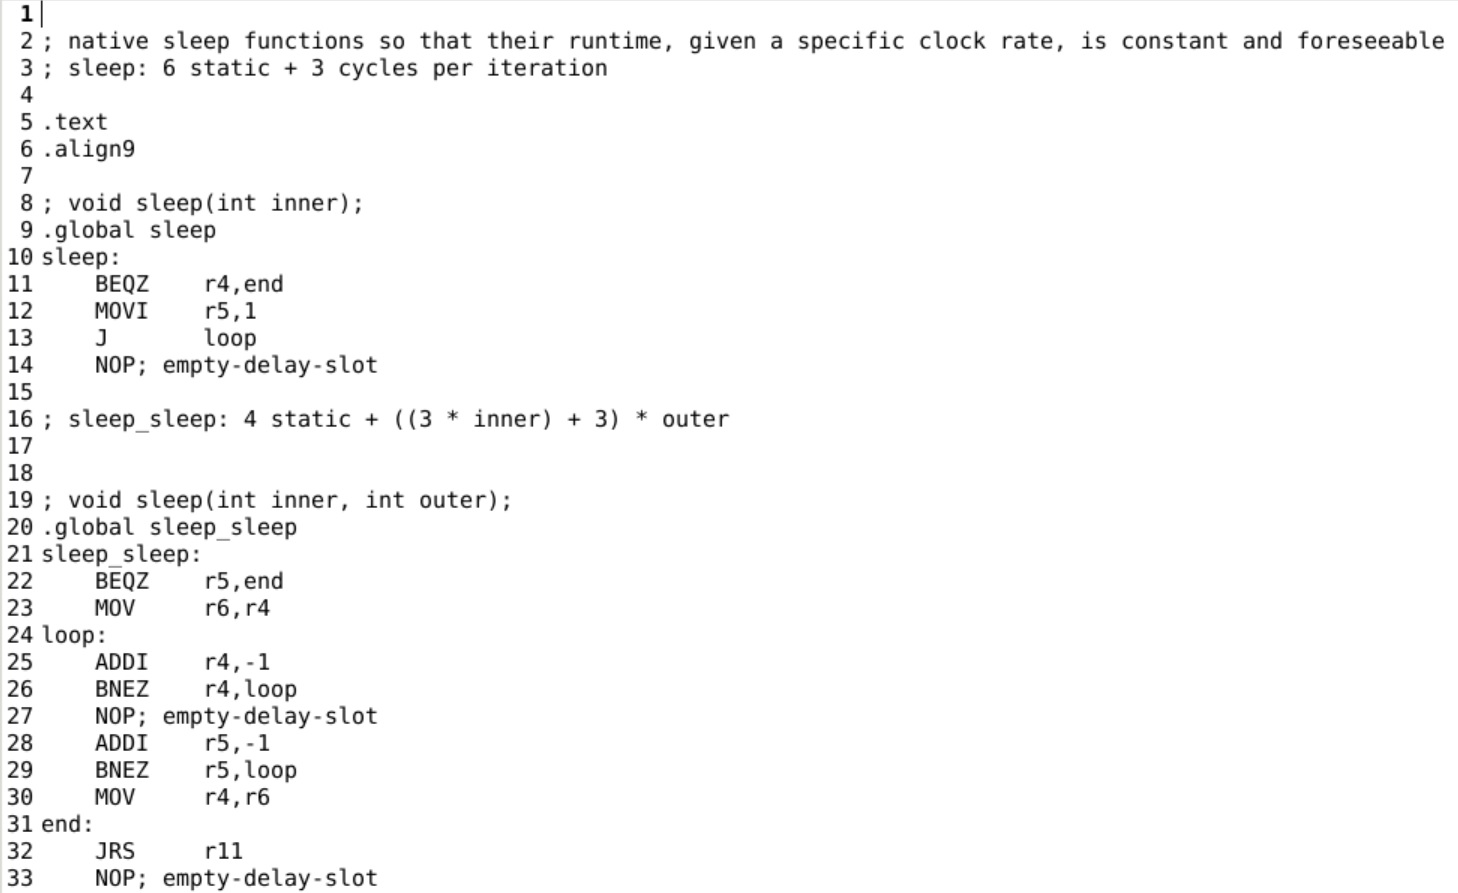
\includegraphics[width=0.9\textwidth]{images/sleep_asm.jpg}
				\caption{sleep and sleep\_sleep assembly, taken from file sleep.s}
				\label{fig:sleep_asm}
			\end{figure}

			According to the description of the sleep procedure, equation \ref{eq:initial_expected_sleep_runtime} shows the expected run time of it in clock cycles. 
			\begin{equation} 
				\label{eq:initial_expected_sleep_runtime}
				delay\_in\_cycles = 6 + 3 \times input\_value
			\end{equation} 
			Looking at figure [\ref{fig:sleep_asm}] it can easily be seen that lines eleven to 14 are causing the first four and lines 32 to 33 the last two static execution cycles, leading the the additional six cycles in the given equation \ref{eq:initial_expected_sleep_runtime}. Looping itself consists of three instructions (lines 25 to 27) and is therefore responsible for having to multiply the input value by three.\\
			The example call of sleep shows that six additional cycles of delay are introduced by a call to sleep. These cycles can not deduced by equation \ref{eq:initial_expected_sleep_runtime}. This is due to the fact that the act of calling the sleep procedure, will cause additional cycles to be spend on the respective operations. These additional cycles are out of the scope of the sleep procedure it self and are therefore not captured by their static runtime component. However, it is notable that the implementation of sleep is intertwined with sleep\_sleep (see fig. [\ref{fig:sleep_asm}]), causing three additional static cycles that should be mentioned by equation \ref{eq:initial_expected_sleep_runtime}. All this leads to the corrected equation \ref{eq:corrected_expected_sleep_runtime}.
			\begin{equation} 
				\label{eq:corrected_expected_sleep_runtime}
				delay\_in\_cycles = 9 + 3 \times input\_value
			\end{equation} 
			As we did not take a look at the assembly of our program, we can not be certain about the remaining three cycles, which lead to the observed overall delay. Assuming that calling sleep is one move (for loading the address) and a jump (with its delay slot), we can see that 15012 cycles of delay for a sleep call with an input value of 5000 are to be expected and can be shown to be correct.

			\paragraph{About sleep\_sleep} % (fold)
			\label{par:about_sleep_sleep}
				As sleep\_sleep shares its inner loop with sleep, the general behaviour of it is the same. However, line 16 of figure [\ref{fig:sleep_asm}] (represented by \ref{eq:sleep_sleep_runtime}) shows that the equation to calculate the expected runtime is different.
				\begin{equation} 
					\label{eq:sleep_sleep_runtime}
					delay\_in\_cycles = 4 + ((3 \times input\_value\_inner) + 3) \times input\_value\_outer
				\end{equation}
				The four static cycles are caused by lines 22 to 23 and lines 32 to 33, representing entry and exit points of the procedure. Three as the factor for the amount of inner loop iterations is directly related to the sleep and also caused by the same lines of code. As the outer loop has to track and manipulate its own counter, three additional cycles are required for each of its iterations.
			% paragraph about_sleep_sleep (end)
		% subsection relation_of_input_to_observed_delay (end)

		\subsection{Results} % (fold)
		\label{sub:results}
			As equations \ref{eq:sleep_sleep_runtime} and \ref{eq:corrected_expected_sleep_runtime} are directly reflected by the code given in figure [\ref{fig:sleep_asm}], the temporal characteristics of a call to sleep or sleep\_sleep can be verified to be true to the expected behaviour. Both procedures could be called in time sensitive programs without introducing none determinism.
		% subsection results (end)
	% section bonus_task_2 (end)
% chapter impl (end)

  %% include further files here ... %

%% Appendix %%%%%%%%%%%%%%%%%%%%%%%%%%%%%%%%%%%%%%%%%%%%%%%%%%%%%%%%%%%
\newpage

\nocite{*}

\printbibliography

\end{document}